\chapter{Object classification with Recurrent Neural Networks}\label{sec:renet}

\section{Introduction}\label{sec:renet_intro}

\emph{Classification} is a broad task that consists in predicting to which
category an input belongs to, out of some $k$ given categories. The system is
usually required to compute a function $f: \RR \to {0, \dots, k-1}$ that
assigns each input to a class. This can be thought as a discrimination task,
where the algorithm is expected to learn similarities and differences between
categories in order to characterize each class.

Some examples of classification are spam detection (classify a message as being
spam or not), credit card fraud detection (identify if a transaction is legit
or not), optical character recognition (OCR) (convert hand-written text to an
electronic document, by classifying each character), speech understanding
(given an utterance from a user, detect the sentence that was pronounced),
medical diagnosis (given the symptoms predict the illness and suggest a cure),
stock trading (determine if a stock should be bought, help or sold, from
current and historical data), shape detection (classify a hand-drawn drawing
from, e.g., a touch screen, as a specific shape) and emotion recognition (given
a text, classify it as being positive, neutral or negative)

\emph{Object recognition} is an instance of this task that takes an image as an
input and is expected to return the id of the main class represented in the
image. This is usually achieved by computing the probability distribution over
the classes -- i.e. the confidence of the algorithm for each class to be the
main class in the scene -- and then picking the one with highest score.

One downside of this method is that small and big mistakes are penalized the
same, i.e., the prediction is considered wrong whether the right class is the
second most probable class in the distribution or is considered extremely
unlikely by the algorithm. For this reason, some competitions such as
e.g.,~ImageNet~\citep{imagenet_cvpr09, ILSVRCarxiv14}, propose multiple
challenges where the top-3 or top-5 guesses are considered, i.e., where an
image is considered correctly predicted if the correct class is in the top
$3$ or $5$ guesses of the network.

Traditionally the computer vision community used to address this task with
heavily hand-engineered systems that typically resorted to finding easily
detectable elements in the image -- such as e.g. edges or corners -- and
computing a descriptor of the surrounding patch. Many detectors~\cite{
dufournaud2000matching,harris1988combined,mikolajczyk2001indexing,
lowe2004distinctive,mikolajczyk2005performance} and descriptors~\cite{
lowe1999object,mikolajczyk2005performance,belongie2002shape} have been proposed
to this end, until in 2012 a deep convolutional neural network shifted the
balance toward learned ANNs indefinitely~\citep{Krizhevsky-2012}. Since then
CNN-based models dominated the object recognition scene.

This chapter presents ReNet, one of the main contributions of this thesis.
The ReNet model is a deep neural network architecture for object recognition,
based on recurrent neural networks. The main idea behind this project was to
propose an alternative to the typical CNN-based approach to object
classification problems. The ReNet model replaces in fact the ubiquitous
convolution+pooling layers of deep CNNs with four recurrent neural networks
that sweep horizontally and vertically in both directions across the image.

The following sections motivate the model in the context of the state of the
art at the time it was conceived, describe the ReNet model in detail and
present the results of its evaluation on three widely-used object recognition
benchmarks, namely  MNIST~\citep{Lecun99objectrecognition},
CIFAR-10~\citep{KrizhevskyHinton2009} and SVHN~\citep{Netzer-wkshp-2011}. The
experiments reveal that the ReNet model performs comparably to convolutional
neural networks on all these datasets, suggesting the potential of RNNs as a
competitive alternative to the conventional deep convolutional neural networks
for image related tasks.


\section{Rationale}
Convolutional neural networks~\cite[CNN,][]{Fukushima80,LeCun89} have become the
method of choice for object recognition after the impressive improvement on the
state of the art of~\cite{Krizhevsky-2012}. CNNs have proved to be successful
at a variety of benchmark problems including, but not limited to, handwritten
digit recognition~\citep[see, e.g.,][]{Ciresan-2012}, natural image
classification~\citep[see, e.g.,][]{Lin2014,Simonyan2015,szegedy2014going},
house number recognition~\citep[see, e.g.,][]{Goodfellow+et+al-ICLR2014a},
traffic sign recognition~\citep[see, e.g.,][]{Ciresan-et-al-2012}, as well as
for speech recognition~\citep[see, e.g.,][]{Hamid2012, sainath2013,
toth2014combining}.  Furthermore, image representations from CNNs trained to
recognize objects on a large set of more than one million
images~\citep{Simonyan2015,szegedy2014going} have been found to be extremely
helpful in performing other computer vision tasks such as image caption
generation~\citep[see, e.g.,][]{Vinyals-et-al-arxiv2014,Xu-et-al-arxiv2015},
video description generation~\citep[see, e.g.,][]{Li2015} and object
localization/detection~\citep[see, e.g.,][]{Sermanet14}.

While the CNN has been especially successful in computer vision, recurrent
neural networks (RNN) have become the method of choice for modeling sequential
data, such as text and sound. Natural language processing (NLP) applications
include language modeling~\citep[see, e.g.,][]{Mikolov-thesis-2012}, and
machine translation~\citep{Sutskever-et-al-NIPS2014,Cho2014,
bahdanau2014neural}. Other popular areas of application include offline
handwriting recognition/generation~\citep{Graves+Schmidhuber-2009,
Graves-et-al-NIPS2007,Graves-arxiv2013} and speech recognition~\citep{
Chorowski-et-al-arxiv2014,Graves+Jaitly-ICML2014}. RNNs have also been used
together with CNNs in speech recognition~\citep{sainath2015}. The recent
revival of RNNs has largely been due to advances in learning
algorithms~\citep{Pascanu+al-ICML2013-small,Martens+Sutskever-ICML2011} and
model architectures~\citep{Pascanu-et-al-ICLR2014,Hochreiter+Schmidhuber-1997,
Cho2014}.

The architecture of ReNet is related and inspired by this earlier work, but
relies on purely uni-dimensional RNNs coupled in a novel way, rather than on a
multi-dimensional RNN. The basic idea behind the ReNet model is to replace each
convolutional layer (with convolution+pooling making up a layer) in the CNN
with four RNNs that sweep over lower-layer features in different directions:
(1) bottom to top, (2) top to bottom, (3) left to right and (4) right to left.
The recurrent layer ensures that each feature activation in its output is an
activation at the specific location \emph{with respect to the whole image}, in
contrast to the usual convolution+pooling layer which only has a local context
window. The lowest layer of the model sweeps over the input image, with
subsequent layers operating on extracted representations from the layer below,
forming a hierarchical representation of the input.

\citet{Graves+Schmidhuber-2009} have demonstrated an RNN-based object
recognition system for offline Arabic handwriting recognition. The main
difference between ReNet and the model of \citet{Graves+Schmidhuber-2009} is
that it uses the usual sequence RNN, instead of the multidimensional RNN. The
way ReNet has been conceived allows in fact to capture the context of the
image without being forced to resort to multidimensional RNNs: the latter two
RNNs (or, equivalently, the last bidirectional RNN), work on the hidden states
computed by the first two RNNs (or the first bidirectional RNN). This allows
to use plain RNNs instead of the more complex multidimensional ones, while
making each output activation of the layer be computed with respect to the
whole input image.

One important consequence of the proposed approach compared to the
multidimensional RNN is that the number of RNNs at each layer scales linearly
with respect to the number of dimensions $d$ of the input image ($2d$). A
multidimensional RNN, on the other hand, requires an exponential number of RNNs
at each layer ($2^d$). Furthermore, the proposed variant is more easily
parallelizable, as each RNN is dependent only along a horizontal or vertical
sequence of patches. This architectural distinction results in the ReNet model
being much more amenable to distributed computing than that
of~\citet{Graves+Schmidhuber-2009}.

\vfill

\section{Model Description}

\begin{figure}
    \centering
    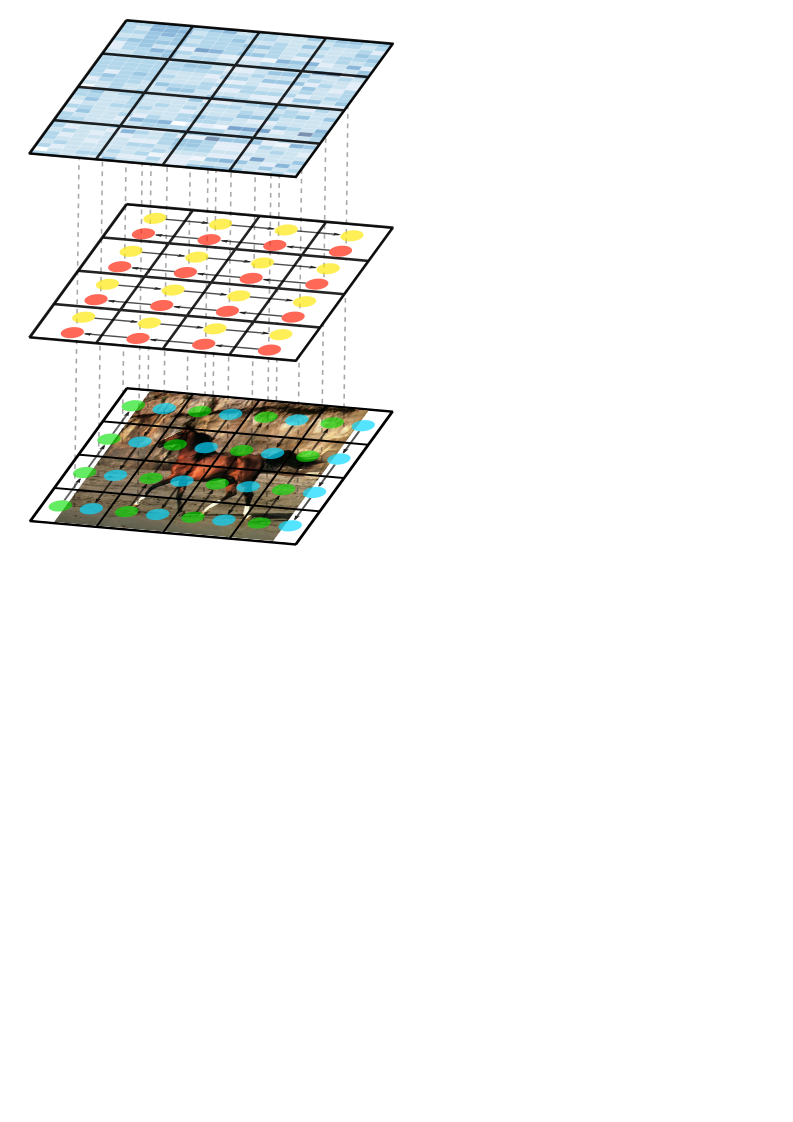
\includegraphics[width=0.3\textwidth]{pdf/renet_first_layer.pdf}
    \caption{A one-layer ReNet}
    \label{fig:networklayer}
    \vspace{-3mm}
\end{figure}

Let us denote by $X=\left\{x_{i,j}\right\}$ the input image or the feature map
from the layer below, where $X \in \RR^{w \times h \times c}$ with $w$, $h$ and
$c$ the width, height and number of channels, or the feature dimensionality,
respectively. Given a receptive field (or patch) size of $w_p \times h_p$, we
split the input image $X$ into a set of $I \times J$ (non-overlapping) patches
$P = \left\{ p_{i,j} \right\}$, where $I = \frac{w}{w_p}$, $J = \frac{h}{h_p}$
and $p_{i,j} \in \RR^{w_p \times h_p \times c}$ is the $(i,j)$-th patch of the
input image. The first index $i$ is the horizontal index and the other index
$j$ is the vertical index.

First, the image is swept vertically with two RNNs, with one RNN working in
a bottom-up direction and the other working in a top-down direction.
Each RNN takes as an input one (flattened) patch at a time and updates its
hidden state, working \emph{along each column} $j$ of the split input image $X$.
\begin{align}
    v^F_{i,j} = f_{\text{VFWD}}(z^F_{i,j-1},p_{i,j}), &\text{ for
    }j=1,\cdots, J\\
    v^R_{i,j} = f_{\text{VREV}}(z^R_{i,j+1},p_{i,j}), &\text{ for
    }j=J,\cdots,1
\end{align}

Note that $f_{\text{VFWD}}$ and $f_{\text{VREV}}$ return the activation of the
recurrent hidden state, and may be implemented either as a simple $\tanh$ layer,
as a gated recurrent layer~\citep{Cho2014} or as a long short-term memory
layer~\citep{Hochreiter+Schmidhuber-1997}.

After this vertical, bidirectional sweep, the intermediate hidden states
$v^F_{i,j}$ and $v^R_{i,j}$ are concatenated at each location $(i,j)$ to get a
composite feature map $V= \left\{ v_{i,j} \right\}_{i=1,\ldots,I}^{
j=1,\ldots,J}$, where $v_{i,j} \in \RR^{2d}$ and $d$ is the number of recurrent
units.  Each $v_{i,j}$ is now the activation of a feature detector at the
location $(i,j)$ with respect to all the patches in the $j$-th column of the
original input ($p_{i, j}$ for all $i$).

Next, the obtained composite feature map $V$ is swept horizontally with two
different RNNs ($f_{\text{HFWD}}$ and $f_{\text{HREV}}$). In a similar manner
as for the vertical sweep, these RNNs work along each row of $V$ and produce an
output feature map $H = \left\{ h_{i,j} \right\}$, where $h_{i,j} \in
\RR^{2d}$. In this representation, each vector $h_{i,j}$ represents the
features of the original image patch $p_{i,j}$ \emph{in the context of the
whole image}.

This is a critical feature of this model, in fact just one layer (to be
precise, two sub-layers) allows to capture the full context of the image,
irrespective of the image size. This is possible thanks to the (potential)
ability of RNNs to store in their memory any information that is relevant to
retain the context of the part of the image that has been processed. The first
two RNNs capture the horizontal dependencies in both directions. By reading
their composite feature map, the second pair of RNNs has access in each
position to a "summary" of the corresponding row. This is processed vertically,
to capture the missing dependencies between rows. This intra- and inter-row
processing results in a final composite feature map where each position is
specific to a pixel (or patch) of the image but has information on the full
image. Conversely, to span over the whole image with CNN-based architectures
would require many more layers, whose number depend on the size of the input
image.

Even if each ReNet layer captures the full input context, it is clearly still
possible to stack multiple ReNet layers on top of each other into a deep
network. Let us denote by $\phi$ the function from the input image (or feature
map) $X$ of one ReNet layer to the output feature map $H$
(see~\autoref{fig:networklayer} for a graphical illustration). It is possible
to compute a composition of functions $\Phi = \phi_1(\phi_2(\phi_3(\dots)))$ by
stacking multiple ReNet layers, to capture increasingly complex features of the
input image.  After any number of recurrent layers are applied to an input
image, the activation at the last recurrent layer may be flattened and fed into
a differentiable classifier to solve an object recognition task. The
experiments on this model, presented in~\autoref{sec:renet_experiments}, used
several fully-connected layers followed by a softmax classifier, as shown
in~\autoref{fig:network}.

The deep ReNet is a smooth, continuous function, and the parameters (those from
the RNNs as well as from the fully-connected layers) can be estimated by the
stochastic gradient descent algorithm with the gradient computed by
backpropagation algorithm~\citep[see, e.g.,][]{BP86} to maximize the
log-likelihood.

\subsection{Differences between LeNet and ReNet}
\label{sec:lenetrenet}

\begin{figure}[h]
    \centering
    \includegraphics[width=0.9\textwidth]{img/lenet5.jpg}
    \caption{The LeNet network}
    \label{fig:lenet}
    \vspace{-3mm}
\end{figure}

This section will use LeNet (see~\autoref{fig:lenet}) to refer to the canonical
convolutional neural network as shown by \citet{LeCun89}. There are many
similarities and differences between the ReNet model and a convolutional neural
network. The main key points of comparison will be highlighted in what follows.

At each layer, both networks apply the same set of filters to patches of the
input image or of the feature map from the layer below. ReNet, however,
propagates information through lateral connections that span across the whole
image, while LeNet exploits local information only. The lateral connections
should help extract a more compact feature representation of the input image at
each layer, which can be accomplished by the lateral connections
removing/resolving redundant features at different locations of the image. This
should allow ReNet resolve small displacements of features across multiple
consecutive patches. Also, the lack of this type of lateral connection in LeNet
may lead to many more levels of convolution+pooling layers in order to detect
redundant features from different parts of the image.

LeNet max-pools the activations of each filter over a small region to achieve
local translation invariance. In contrast, the proposed ReNet does not use any
pooling due to the existence of learned lateral connections. The lateral
connection in ReNet can emulate the local competition among features induced by
the max-pooling in LeNet.  This does not mean that it is not possible to use
max-pooling in ReNet. The use of max-pooling in the ReNet could be helpful in
reducing the dimensionality of the feature map, resulting in lower computational
cost.

Max-pooling as used in LeNet may prove problematic when building a
convolutional autoencoder whose decoder is an inverse\footnote{
    All the forward arrows from the input to the output in the original LeNet
    are reversed.
}
of LeNet, as the max operator is not invertible. The proposed
ReNet is end-to-end smooth and differentiable, making it more suited to be used
as a decoder in the autoencoder or any of its probabilistic variants~\citep[see,
e.g.,][]{Kingma+Welling-ICLR2014}.

In some sense, each layer of the ReNet can be considered as a variant of a usual
convolution+pooling layer, where pooling is replaced with lateral connections,
and convolution is done without any overlap. Similarly, \citet{Springenberg2014}
recently proposed a variant of a usual LeNet which does not use any pooling.
They used convolution with a larger stride to compensate for the lack of
dimensionality reduction by pooling at each layer. However, this approach still
differs from the proposed ReNet in the sense that each feature activation at a
layer is only with respect to a subset of the input image rather than the whole
input image.

The main disadvantage of ReNet is that it is not easily parallelizable, due to
the sequential nature of the recurrent neural network (RNN). LeNet, on the other
hand, is highly parallelizable due to the independence of computing activations
at each layer. The introduction of sequential, lateral connections, however, may
result in more efficient parametrization, requiring a smaller number of
parameters with overall fewer computations, although this needs to be further
explored. Note that this limitation on parallelization applies only to model
parallelism, and any technique for data parallelism may be used for both the
proposed ReNet and the LeNet.

\section{Experiments}\label{sec:renet_experiments}

\subsection{Datasets}

The ReNet model has been evaluated on three widely-used benchmark datasets;
MNIST, CIFAR-10 and the Street View Housing Numbers (SVHN). This section
describes each dataset in detail.

\paragraph{MNIST}

\begin{figure}[h]
    \centering
    \includegraphics[width=0.5\textwidth]{img/mnist_digits.png}
    \caption{Some digits from the MNIST dataset}
    \label{fig:mnist_digits}
\end{figure}

The MNIST dataset~\citep{Lecun99objectrecognition} consists of 70,000
handwritten digits from 0 to 9, centered on a $28\times 28$ square
canvas~(see~\autoref{fig:mnist_digits} for some samples). Each pixel represents
the grayscale in the range of $\left[0, 255\right]$.\footnote{Each pixel has
been scaled to $[0, 1]$ by dividing it with $255$.} It is customary to split
this dataset into 50,000 training samples, 10,000 validation samples and 10,000
test samples. For a fair comparison, the results reported
in~\autoref{sec:renet_results} were obtained following the standard split.

\paragraph{CIFAR-10}

\begin{figure}[h]
    \centering
    \includegraphics[width=0.5\textwidth]{img/cifar-10.png}
    \caption{Some samples of the 10 classes of the CIFAR-10 dataset}
    \label{fig:cifar}
\end{figure}

The CIFAR-10 dataset~\citep{KrizhevskyHinton2009} is a curated subset of the 80
million tiny images dataset~(see~\autoref{fig:cifar} for some samples),
originally released by \citet{Torralba+Fergus+Freeman-2008}. CIFAR-10 contains
60,000 images each of which belongs to one of ten categories: airplane,
automobile, bird, cat, deer, dog, frog, horse, ship and truck. Each image is 32
pixels wide and 32 pixels high with 3 color channels (red, green and blue.)
Following the standard procedure, in the reported experiments the dataset
was split into 40,000 training, 10,000 validation and 10,000 test samples.
Furthermore, zero-phase component analysis (ZCA) was applied and the each pixel
was normalized to have zero-mean and unit-variance across the training samples,
as suggested by \citet{KrizhevskyHinton2009}.

\paragraph{Street View House Numbers}

\begin{figure}[h]
    \centering
    \includegraphics[width=0.5\textwidth]{img/SVHN.png}
    \caption{Some samples of housing numbers from the SVHN dataset}
    \label{fig:svhn}
\end{figure}

The Street View House Numbers (SVHN) dataset~\citep{Netzer-wkshp-2011} consists
of cropped images representing house numbers captured by Google StreetView
vehicles as a part of the Google Maps mapping process. These images consist of
digits 0 through 9 with values in the range of [0, 255] in each of 3
red-green-blue color channels~(see~\autoref{fig:svhn} for some samples). Each
image is 32 pixels wide and 32 pixels high giving a sample dimensionality (32,
32, 3). The number of samples used for the training, validation, and test sets
is 543,949, 60,439, and 26,032 respectively. Each pixel was normalized to have
zero-mean and unit-variance across the training samples.

\subsection{Data Augmentation}

It has been long known that augmenting training data often leads to better
generalization~\citep[see, e.g.,][]{Krizhevsky-2012}. The results reported
in~\autoref{sec:renet_results} were all obtained employing two primary data
augmentations: {\it flipping} and {\it shifting}.

For the flipping data augmentation, the model was presented with samples that
were either flipped horizontally with 25\% chance, or vertically with 25\%
chance, or left unchanged. This technique allows the model to observe ``mirror
images'' of the original images of the dataset during training, increasing the
amount of training data. On SVHN and MNIST only horizontal flipping was used
to prevent the case were an image labelled $6$ is flipped in both direction,
becoming a $9$.

In the case of shifting two policies were adopted. The images were either
shifted by 2 pixels to the left (25\% chance), 2 pixels to the right (25\%
chance) or left as they were. After this first processing, the images were
further shifted either by 2 pixels to the top (25\% chance), 2 pixels to the
bottom (25\% chance) or left as they were. This two-step procedure makes the
model more robust to slight shifting of an object in the image. The shifting
was done without pre-padding the borders of the image, but rather preserving
the original size by dropping the pixels which are shifted out of the input
and shifting in zeros on the opposite side.

The choice of whether to apply these augmentation procedures on each dataset
was chosen on a per-case basis in order to maximize validation performance.

\begin{figure}[t]
    \centering
    \includegraphics[height=.14\textheight,width=\columnwidth]{pdf/renet_svhn.pdf}
    \caption{The ReNet network used for SVHN classification}
    \label{fig:network}
\end{figure}

\subsection{Model Architectures}

The principal parameters that define the architecture of the ReNet model are
the number of ReNet layers ($N_{\text{RE}}$), their corresponding receptive
field sizes ($w_p \times h_p$) and feature dimensionality ($d_{\text{RE}}$),
the number of fully-connected layers ($N_{\text{FC}}$) and their corresponding
numbers ($d_{\text{FC}}$) and types ($f_{\text{FC}}$) of hidden units.

Table~\ref{tbl:architectures} summarizes the settings of these hyperparameters
that performed best on the validation set of the studied datasets.
\autoref{fig:network} is a graphical illustration of the model selected with
this metric for the SVHN dataset.

\begin{table}[t]
    \centering
    \begin{tabular}{l || c | c | c }
        & MNIST & CIFAR-10 & SVHN \\
        \hline
        \hline
    $N_{\text{RE}}$ & 2 & 3 & 3 \\
        \hline
        $w_p \times h_p$ & $[2\times 2]$--$[2 \times 2]$ & $[2\times 2]$--$[2 \times 2]$--$[2
        \times 2]$ & $[2\times 2]$--$[2 \times 2]$--$[2 \times 2]$ \\
        \hline
    $d_{\text{RE}}$ & 256--256 & 320--320--320 & 256--256--256 \\
        \hline
    $N_{\text{FC}}$ & 2 & 1 & 2 \\
        \hline
    $d_{\text{FC}}$ & 4096--4096 & 4096 & 4096--4096 \\
        \hline
    $f_{\text{FC}}$ & $\max(0, x)$ & $\max(0,x)$ & $\max(0,x)$ \\
        \hline
    Flipping & no & yes & no \\
        \hline
    Shifting & yes & yes & yes \\
    \end{tabular}
    \caption{Model architectures used in the experiments. Each row shows
             respectively the number of ReNet layers, the size of the patches,
             the number of neurons of each ReNet layer, the number of fully
             connected layers, the number of neurons of the fully connected
             layers, their activation function and the data augmentation
             procedure employed.}
    \label{tbl:architectures}
\end{table}

\subsubsection{Training}

All the networks have been trained using a recently proposed adaptive learning
rate algorithm, called Adam~\citep{Kingma2014}. In order to reduce overfitting
dropout~\citep{Srivastava14} was applied after each layer, including both the
ReNet layers (after the horizontal and vertical sweeps) and the fully-connected
layers. The input layer was also corrupted by masking out each pixel with
probability $0.2$. Finally, each optimization run was early stopped based
on validation error.

Note that the results reported in~\autoref{sec:renet_results} were obtained
without retraining on the joint training and validation sets. This is a common
technique exploited by many works in the literature to boost the performance
of the best model, selected after a full training on the training set early
stopping on the validation performance. There is no reason not to think that
this would further improve the reported results, but this work was mainly
conceived as a proof of concept rather than to stress on the absolute
performance. This, as well as e.g., ensembling multiple models, can be seen as
one of the many potential areas of exploration for further work in case maximum
performance is sought.

\begin{table}[ht]
    \centering

    \begin{minipage}{0.45\textwidth}
        \centering

        \begin{tabular}{l |  l}
            Test Error & Model  \\
            \hline
0.28\% & \citep{DBLP:conf/icml/WanZZLF13}$\star$ \\
0.31\% & \citep{DBLP:journals/corr/Graham14}$\star$ \\
0.35\% & \citep{DBLP:journals/corr/abs-1003-0358} \\
0.39\% & \citep{DBLP:conf/nips/MairalKHS14}$\star$ \\
0.39\% & \citep{DBLP:journals/corr/LeeXGZT14}$\star$ \\
0.4\% & \citep{DBLP:conf/icdar/SimardSP03}$\star$ \\
0.44\% & \citep{DBLP:journals/corr/Graham14a}$\star$ \\
0.45\% & \citep{Goodfellow2013}$\star$ \\
\bf{0.45\%} & \bf{ReNet} \\
0.47\% & \citep{Lin2014}$\star$ \\
0.52\% & \citep{DBLP:journals/pami/AzzopardiA13} \\
        \end{tabular}

        \vspace{2mm}
        (a) MNIST
    \end{minipage}
    \hfill
    \begin{minipage}{0.45\textwidth}
        \centering

        \begin{tabular}{l |  l}
            Test Error & Model  \\
            \hline
4.5\% & \citep{DBLP:journals/corr/Graham14a}$\star$ \\
6.28\% & \citep{DBLP:journals/corr/Graham14}$\star$ \\
8.8\% & \citep{Lin2014}$\star$ \\
9.35\% & \citep{Goodfellow2013}$\star$ \\
9.39\% & \citep{DBLP:journals/corr/SpringenbergR13}$\star$ \\
9.5\% & \citep{DBLP:conf/nips/SnoekLA12}$\star$ \\
11\% & \citep{Krizhevsky-2012}$\star$ \\
11.10\% & \citep{DBLP:conf/icml/WanZZLF13}$\star$ \\
\bf{12.35\%} & \bf{ReNet} \\
15.13\% & \citep{DBLP:journals/corr/abs-1301-3557}$\star$ \\
15.6\% & \citep{DBLP:journals/corr/abs-1207-0580}$\star$ \\
        \end{tabular}

        \vspace{2mm}
        (b) CIFAR-10
    \end{minipage}

    \vspace{4mm}
    \begin{minipage}{0.45\textwidth}
        \centering
        \begin{tabular}{l |  l}
            Test Error & Model  \\
            \hline
1.92\% & \citep{DBLP:journals/corr/LeeXGZT14}$\star$ \\
2.23\% & \citep{DBLP:conf/icml/WanZZLF13}$\star$ \\
2.35\% & \citep{Lin2014}$\star$ \\
\bf{2.38\%} & \bf{ReNet} \\
2.47\% & \citep{Goodfellow2013}$\star$ \\
2.8\% & \citep{DBLP:journals/corr/abs-1301-3557}$\star$ \\
        \end{tabular}

        \vspace{2mm}
        (c) SVHN
    \end{minipage}
    \hfill
    \begin{minipage}{0.51\textwidth}
        \caption{Generalization errors obtained by the proposed ReNet along
            with those reported by previous works on each of the three
            datasets. For a fair comparison, only results obtained by a single
            model are listed, i.e., no ensembling of multiple models. In the
            case of SVHN, only models trained on the Format 2 (cropped digits)
            dataset are reported. $\star$ denotes a convolutional neural
            network.}
        \label{tbl:result}
    \end{minipage}
\end{table}

\subsection{Results}\label{sec:renet_results}
Table~\ref{tbl:result}, presents the results of ReNet on three datasets, along
with previously reported results.

It is clear that ReNet performs comparably to deep convolutional neural
networks which are the {\it de facto} standard for object recognition. This
suggests that ReNet is a viable alternative to convolutional neural networks
(CNN), even on tasks where CNNs have historically dominated. However, it is
important to notice that ReNet does not outperform state-of-the-art
convolutional neural networks on any of the three benchmark datasets, which
calls for more research in the future.

\section{Conclusions/Discussion}

\paragraph{Choice of Recurrent Units}
Note that the proposed architecture is independent of the chosen recurrent
units. The preliminary experiments on this model showed that gated recurrent
units, either the GRU or the LSTM, outperform a usual sigmoidal unit (affine
transformation followed by an element-wise sigmoid function.) This indirectly
confirms that the model utilizes long-term dependencies across an input image,
and the gated recurrent units help capture these dependencies.

\paragraph{Analysis of the Trained ReNet}
In this paper, we evaluated the proposed ReNet only quantitatively. However, the
accuracies on the test sets do not reveal what kind of image structures the
ReNet has captured in order to perform object recognition. Due to the large
differences between ReNet and LeNet discussed in
Sec.~\ref{sec:lenetrenet}, we expect that the internal behavior of ReNet
will differ from that of LeNet significantly. Further investigation along
the line of \citep{ZeilerFergus14} will be needed, as well exploring ensembles
which combine RNNs and CNNs for bagged prediction.

\paragraph{Computationally Efficient Implementation}
As discussed in Sec.~\ref{sec:lenetrenet}, the proposed ReNet is less
parallelizable due to the sequential nature of the recurrent neural network
(RNN). Although this sequential nature cannot be addressed directly, our
construction of ReNet allows the forward and backward RNNs to be run
independently from each other, which allows for parallel computation.
Furthermore, we can use many parallelization tricks widely used for training
convolutional neural networks such as parallelizing fully-connected layers
~\citep{krizhevsky2014one}, having separate sets of kernels/features in
different processors~\citep{Krizhevsky-2012} and exploiting data parallelism.


% \begin{table}[h]
% \begin{tabular}{ll}
% 0.35\% & Deep Big Simple Neural Nets Excel on Handwritten Digit Recognition \citep{DBLP:journals/corr/abs-1003-0358} \\
% 0.39\% & Convolutional Kernel Networks \citep{DBLP:conf/nips/MairalKHS14} \\
% 0.39\% & Deeply-Supervised Nets \citep{DBLP:journals/corr/LeeXGZT14} \\
% 0.4\% & Best Practices for Convolutional Neural Networks Applied to Visual Document Analysis \citep{DBLP:conf/icdar/SimardSP03} \\
% 0.45\% & Maxout Networks \citep{Goodfellow2013} \\
% \bf{0.45\%} & \bf{ReNet} \\
% 0.47\% & Network in Network \citep{Lin2014} \\
% 0.52\% & Trainable COSFIRE filters for keypoint detection and pattern recognition \citep{DBLP:journals/pami/AzzopardiA13} \\
% \end{tabular}
% \end{table}
%
% MNIST (talk about why we don't compare to dropconnect/multicolumn?)
%
% CIFAR-10 (briefly mention ZCA, flipping, pixel shift)
% \begin{table}[h]
% \begin{tabular}{ll}
% 8.8\% & Network In Network \citep{Lin2014} \\
% 9.32\% & Regularization of Neural Networks using DropConnect \citep{DBLP:conf/icml/WanZZLF13} \\
% 9.35\% & Maxout Networks \citep{Goodfellow2013} \\
% 9.39\% & Improving Deep Neural Networks with Probabilistic Maxout Units \citep{DBLP:journals/corr/SpringenbergR13} \\
% 9.5\% & Practical Bayesian Optimization of Machine Learning Algorithms \citep{DBLP:conf/nips/SnoekLA12} \\
% 11\% & ImageNet Classification with Deep Convolutional Neural Networks \citep{Krizhevsky-2012} \\
% 11.21\% & Multi-Column Deep Neural Networks for Image Classification \citep{Ciresan-2012} \\
% \bf{12.35\%} & \bf{ReNet} \\
% 15.13\% & Stochastic Pooling for Regularization of Deep Convolutional Neural Networks \citep{DBLP:journals/corr/abs-1301-3557} \\
% 15.6\% & Improving neural networks by preventing co-adaptation of feature detectors \citep{DBLP:journals/corr/abs-1207-0580} \\
% \end{tabular}
% \end{table}
%
% SVHN (briefly mention flipping, pixel shift)
% \begin{table}[h]
% \begin{tabular}{ll}
% 1.92\% & Deeply Supervised Nets \citep{DBLP:journals/corr/LeeXGZT14} \\
% 1.94\% & Regularization of Neural Networks using DropConnect \citep{DBLP:conf/icml/WanZZLF13} \\
% 2.16\% & Multi-digit Number Recognition from Street View Imagery using Deep Convolutional Neural Networks \citep{Goodfellow+et+al-ICLR2014a} \\
% 2.35\% & Network in Network \citep{Lin2014} \\
% \bf{2.38\%} & \bf{ReNet} \\
% 2.47\% & Maxout Networks \citep{Goodfellow2013} \\
% 2.8\% & Stochastic Pooling for Regularization of Deep Convolutional Neural Networks \citep{DBLP:journals/corr/abs-1301-3557} \\
% \end{tabular}
% \end{table}
